% Template per generare 

\documentclass[a4paper,11pt]{article}
\usepackage{lmodern}
\renewcommand*\familydefault{\sfdefault}
\usepackage{sfmath}
\usepackage[utf8]{inputenc}
\usepackage[T1]{fontenc}
\usepackage[italian]{babel}
\usepackage{indentfirst}
\usepackage{graphicx}
\usepackage{tikz}
\usepackage{listings}
\newcommand*\circled[1]{\tikz[baseline=(char.base)]{
		\node[shape=circle,draw,inner sep=2pt] (char) {#1};}}
\usepackage{enumitem}
% \usepackage[group-separator={\,}]{siunitx}
\usepackage[left=2cm, right=2cm, bottom=3cm]{geometry}
\frenchspacing

\newcommand{\num}[1]{#1}

% Macro varie...
\newcommand{\file}[1]{\texttt{#1}}
\renewcommand{\arraystretch}{1.3}
\newcommand{\esempio}[2]{
\noindent\begin{minipage}{\textwidth}
\begin{tabular}{|p{8cm}|p{8cm}|}
	\hline
      \textbf{\file{input (da stdin)}} & \textbf{\file{output (su stdout)}}\\
	\hline
	\tt \small #1 &
	\tt \small #2 \\
	\hline
\end{tabular}
\end{minipage}
}

% Dati del task
\newcommand{\gara}{Esame Algoritmi 2019-07-30}
\newcommand{\nome}{Trascodifica di alberi ordinati - discendenza in pre o post-order?}
\newcommand{\nomebreve}{tree\_transcode\_disc}

\begin{document}
% Intestazione
\noindent{\Large \gara}
\vspace{0.5cm}

\noindent{\Huge \textbf \nome~(\texttt{\nomebreve})}

% Descrizione del task
\section*{Descrizione del problema}

Un \emph{albero ordinato} consta di un \emph{nodo radice} e di una sequenza finita (eventualmente vuota) di \emph{figli} della radice, che sono a loro volta alberi ordinati.
Su ciascun nodo dell'albero ordinato in figura compare il numero dei suoi discendenti (incluso il nodo stesso). Per convenzione, la radice viene disegnata in cima (cio\`e al contrario rispetto agli alberi veri).

\begin{figure}[h!]
  \centering
    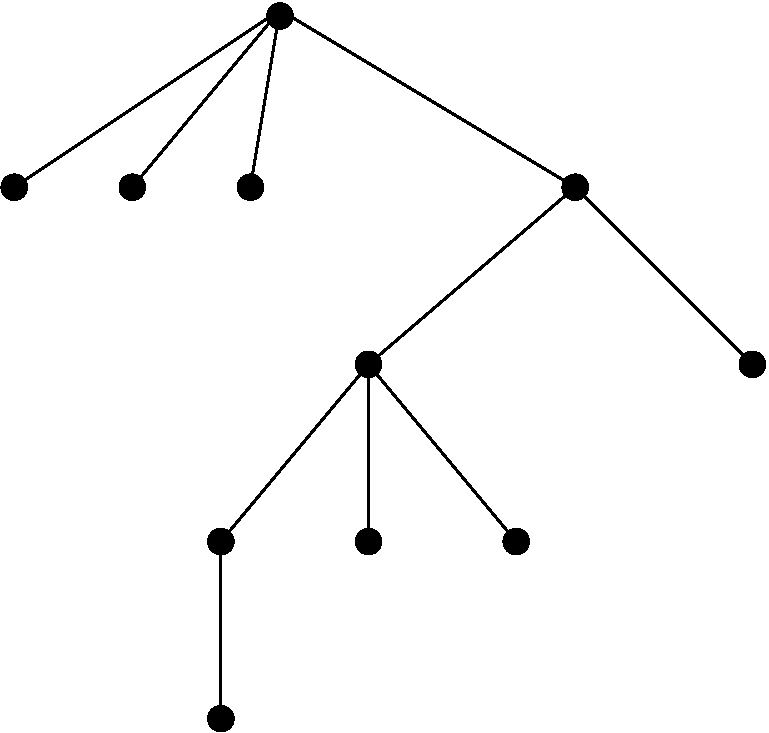
\includegraphics[scale=0.5]{figs/fig2.pdf}
%      \quad \quad \quad \quad
%    \includegraphics[scale=0.4]{figs/fig3.pdf}
%    \caption{Un albero. Il nodo radice è quello più in alto. Per ogni nodo viene riportato il numero dei suoi discendenti (incluso il nodo stesso).}
\end{figure}

Proponiamo due possibili modi di codificare un albero come una sequenza di numeri naturali. Il primo numero della sequenza è~$1$ oppure~$2$
a seconda del sistema di codifica scelto.\\

\noindent
{\bf Codifica~1:}
Una sequenza di tanti numeri naturali quanti sono i nodi dell'albero. 
L'albero viene descritto dicendo quanti discendenti ha la radice (in questo caso 11) e poi descrivendo uno a uno, nell'ordine da sinistra a destra, i sottoalberi radicati nei figli della radice, uno per figlio. Ad esempio, l'albero in figura sarebbe identificato dalla seguente sequenza:
\[
1\,\,\,11\,\,\,7\,\,\,1\,\,\,5\,\,\,1\,\,\,1\,\,\,2\,\,\,1\,\,\,1\,\,\,1\,\,\,1
\]	

Infatti, l'albero ha 11 nodi in tutto, ossia 11 sono i discendenti della radice (ogni nodo si considera discendente di se stesso), per cui il primo numero dopo lo specificatore di formato ($1$) \`e $11$. A questo $11$ segue poi subito la sequenza $7\,\,\,1\,\,\,5\,\,\,1\,\,\,1\,\,\,2\,\,\,1$, che \`e la descrizione del primo sottoalbero, mentre gli ultimi tre sottoalberi sono ciascuno descritti da un solo $1$ (dato che non hanno alcun figlio).

\noindent
{\bf Codifica~2:}
Una sequenza di tanti numeri naturali quanti sono i nodi dell'albero. 
Di nuovo, l'albero viene descritto specificando il numero di discendenti di ciascun nodo, ma questa volta l'ordine in cui i nodi parlano è diverso:
per descrivere un albero, prima si descrivono uno alla volta i sottoalberi dei figli della radice (ossia quelli radicati nei vari figli della radice), e solo poi parla la radice.
Ad esempio, l'albero in figura sarebbe identificato dalla seguente sequenza:
\[
2\,\,\,1\,\,\,1\,\,\,1\,\,\,1\,\,\,2\,\,\,5\,\,\,7\,\,\,1\,\,\,1\,\,\,1\,\,\,11
\]	
In pratica, ciascun nodo parla solo in chiusura del sottoalbero di cui egli è radice.
A parte questa differenza, l'ordine in cui ogni sottoalbero viene aperto e chiuso nella visita è lo stesso che per la Codifica~1, e segue l'ordinamento sui figli come fissato su ciascun nodo. 


% Input
\section*{Dati di input}

L'input deve avvenire da stdin, da dove il vostro programma legge una sola riga contenente la codifica di un albero offerta secondo il primo o secondo formato.

% Output
\section*{Dati di output}

L'output deve avvenire su stdout, dove il vostro programma deve restituisce una sola riga: la codifica dello stesso albero nell'altro formato.

% Esempi
\section*{Esempio di input/output}
\esempio{
1 11 7 1 5 1 1 2 1 1 1 1
}{
2 1 1 1 1 2 5 7 1 1 1 11
}


\section*{Esempio di input/output}
\esempio{
2 1 1 1 1 2 5 7 1 1 1 11
}{
1 11 7 1 5 1 1 2 1 1 1 1
}

% Assunzioni
\section*{Assunzioni}
\begin{itemize}[nolistsep, noitemsep]
\item dove $n$ \`e il numero di nodi dell'albero,
      vale sempre che $1 \le n \le 1\,000\,000 $;
\item tempo limite: un secondo.
\end{itemize}

% Subtasks
\section*{Subtask}
Un totale di $100$ punti \`e ripartito su $11$ subtask.
Il subtask coi casi di esempio non dà punti.
\begin{itemize}
\item \textbf{Subtask 1 [0 punti]:} l'esempio del testo.
\item \textbf{Subtask x+2 [10 punti]:} ogni nodo ha massimo un figlio.
\item \textbf{Subtask x+3 [10 punti]:} ogni nodo ha massimo due figli.
\item \textbf{Subtask x+4 [10 punti]:} $N \le 10$.
\item \textbf{Subtask x+5 [10 punti]:} $N \le 1000$.
\item \textbf{Subtask x+6 [10 punti]:} $N \le 1\,000\,000$.
\end{itemize}
Come interpretare $x$: alcune istanze ($x=0$) chiedono di passare dalla prima alla seconda codifica,
altre ($x=5$) chiedono di passare dalla seconda alla prima codifica.


\end{document}
